\section{随机变量及分布 II}

\subsection{连续型随机变量}

\begin{definition}
    设 $X$ 是一个随机变量，若存在非负可积函数 $f(x)$ 使得
    $$
    F(x) = \int_{- \infty}^{x} f(t) \dd{t}
    $$
    其中 $F(x)$ 是它的分布函数，那么称 $X$ 是\textbf{连续型随机变量}，$f(x)$ 是它的\textbf{概率密度函数}。
\end{definition}

概率密度函数满足下面的性质：
\begin{itemize}
    \item $f(x) \ge 0$；
    \item $\displaystyle\int_{- \infty}^{+ \infty} f(x) \dd{x} = 1$；
    \item $\displaystyle \prob{a < X < b} = \int_{a}^{b} f(x) \dd{x}$。
\end{itemize}

\subsection{连续型随机变量的分布}

\subsubsection{均匀分布}

\begin{definition}
    若 $X$ 的概率密度函数为
    $$
    f(x) = \begin{cases}
        \frac{1}{b - a} &, a \le x \le b \\
        0 &, \text{otherwise}
    \end{cases}
    $$
    那么称 $X$ 满足\textbf{均匀分布}。
\end{definition}

当 $X$ 满足均匀分布的时候，对于任意 $(c, d) \subseteq (a, b)$，都有 $\prob{c < X < d} = d - c$。概率只和区间长度有关，和区间位置无关。

\subsection{指数分布}

\begin{definition}
    若 $X$ 的概率密度函数为
    $$
    f(x) = \begin{cases}
        \lambda \E^{-\lambda x} &, x > 0 \\
        0 &, \text{otherwise}
    \end{cases}
    $$
    那么称 $X$ 满足\textbf{指数分布}。
\end{definition}

对 $f(x)$ 进行积分，可以得到指数分布的分布函数为
$$
F(x) = \begin{cases}
    1 - \E^{-\lambda x} &, x > 0 \\
    0 &, \text{otherwise}
\end{cases}
$$

\subsubsection{正态分布}

先引入 Euler-Poission 积分
$$
\int_{- \infty}^{+ \infty} \E^{-x^2} \dd{x} = \sqrt{\pi}
$$
证明如下，记原积分为 $I$：
$$
\begin{aligned}
    I^2 & = \ab(\int_{-\infty}^{+ \infty} \E^{-x^2} \dd{x}) \\
    & = \iint_{\mathbb{R}^2} \E^{-x^2 - y^2} \dd{x} \dd{y} \\
    & = \int_{0}^{2\pi} \dd{\theta} \int_{0}^{+\infty} \E^{-r^2} r \dd{r} \\
    & = 2\pi \cdot \ab[-\frac{1}{2} \E^{-r^2}]_{0}^{+\infty} \\
    & = \pi
\end{aligned}
$$
因此 $I = \sqrt{\pi}$。

\begin{definition}[正态分布]
    若随机变量 $X$ 的概率密度函数为
    $$
    f(x) = \frac{1}{\sqrt{2\pi} \sigma} \E^{-\frac{(x - \mu)^2}{2 \sigma^2}}
    $$
    那么称 $X$ 满足\textbf{正态分布}，记做 $X \sim N(\mu, \sigma^2)$。
\end{definition}

正态分布满足下面的性质：

\begin{itemize}
    \item $f(x)$ 在 $x = \mu$ 取得最大值；
    \item $f(x)$ 在 $x = \mu \pm \sigma$ 时取到拐点；
    \item $X$ 的平均数为 $\mu$，方差为 $\sigma$。
\end{itemize}

\subsection{作业}

\begin{problem}
    习题 2.17
    \begin{solution}
        \begin{enumerate}
            \item[\textbf{1)}] 由题可得，$\prob{X = 0} = 1 - p,\ \prob{X = 1} = p$，因此：
            $$
            F(x) = \prob{X \le x} = \begin{cases}
                0 &, x < 0 \\
                1 - p &, 0 \le x < 1, \\
                1 &, x \ge 1
            \end{cases}
            $$
            其图像为：
            \begin{figure}[H]
                \centering
                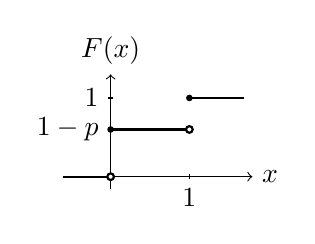
\begin{tikzpicture}
                    % 坐标轴
                    \draw[->] (-0.6,0) -- (1.8,0) node[right] {$x$};
                    \draw[->] (0,-0.15) -- (0,1.3) node[above] {$F(x)$};

                    % 刻度
                    \draw (1,0.03) -- (1,-0.03) node[below] {$1$};
                    \draw (0.03,1) -- (-0.03,1) node[left] {$1$};
                    \draw (0.03,0.6) -- (-0.03,0.6) node[left] {$1-p$};

                    % x < 0: F(x) = 0
                    \draw[thick] (-0.6,0) -- (0,0);
                    \draw[fill=white, thick] (0,0) circle (1.2pt);

                    % 0 <= x < 1: F(x) = 1-p
                    \draw[thick] (0,0.6) -- (1,0.6);
                    \fill (0,0.6) circle (1.2pt);
                    \draw[fill=white, thick] (1,0.6) circle (1.2pt);

                    % x >= 1: F(x) = 1
                    \draw[thick] (1,1) -- (1.7,1);
                    \fill (1,1) circle (1.2pt);
                \end{tikzpicture}
            \end{figure}

            \item[\textbf{2)}]
            $$
            F(x) = P(X \le x) = \begin{cases}
                0 &, x < 3 \\
                \frac{1}{10} &, 3 \le x < 4 \\
                \frac{2}{5} &, 4 \le x < 5 \\
                1 &, x \ge 1
            \end{cases}
            $$
        \end{enumerate}
    \end{solution}
\end{problem}

\begin{problem}
    习题 2.18
    \begin{solution}
        由题可知 $X$ 服从均匀分布，因此
        $$
        F(x) = P(X \le x) = \begin{cases}
            0 &, x < 0 \\
            \frac{x}{a} &, 0 \le x < 1 \\
            1 &, x \ge 1
        \end{cases}
        $$
    \end{solution}
\end{problem}

\begin{problem}
    习题 2.19
    \begin{solution}
        记 $F_X(+ \infty) = \lim\limits_{x \to +\infty} F_X(x) = 1$。
        \begin{enumerate}
            \item[\textbf{1)}] $P = F_X(3) - F_X(0) \approx 0.70$；
            \item[\textbf{2)}] $P = F_X(+ \infty) - F_X(4) \approx 0.20$；
            \item[\textbf{3)}] $P = F_X(4) - F(3) \approx 0.10$；
            \item[\textbf{4)}] $P = (F_X(3) - F_X(0)) + (F_X(+ \infty) - F_X(4)) \approx 0.90$；
            \item[\textbf{5)}] $P = 0$。
        \end{enumerate}
    \end{solution}
\end{problem}

\begin{problem}
    习题 2.20
    \begin{solution}
        \begin{enumerate}
            \item[\textbf{1)}]
            $$
            \begin{gathered}
                \prob{X < 2} = F_X(2 - 0) = \ln 2 \\
                \prob{0 < X \le 3} = F_X(3) - F_X(0) = 1 \\
                \prob{2 < X < \frac{5}{2}} = F_X(\frac{5}{2} - 0) - F_X(2) = \ln \frac{5}{4}
            \end{gathered}
            $$
            \item[\textbf{2)}]
            $$
            f_X(x) = \dv{F_X}{x} = \begin{cases}
                0 &, x < 1 \\
                \frac{1}{x} &, 1 \le x < \E \\
                0 &, x \ge \E
            \end{cases}
            $$
        \end{enumerate}
    \end{solution}
\end{problem}

\begin{problem}
    习题 2.21
    \begin{enumerate}
        \item[\textbf{1)}]
        $$
        F(x) = \prob{X \le x} = \int_{- \infty}^{x} f(t) \dd{t} = \begin{cases}
            0 &, x < 1 \\
            x + \frac{1}{x} - 2 &, 1 \le x < 2 \\
            1 &, x \ge 2
        \end{cases}
        $$
        \item[\textbf{2)}]
        $$
        F(X) = \prob{X \le x} = \int_{- \infty}^{x} f(t) \dd{t} = \begin{cases}
            0 &, x < 0 \\
            \frac{1}{2} x^2 &, 0 \le x < 1 \\
            2x - \frac{1}{2} x^2 - 1 &, 1 \le x < 2 \\
            1 &, x \ge 2
        \end{cases}
        $$
        \begin{figure}[H]
            \centering
            \begin{tikzpicture}
                % 分布函数 F(x)
                \begin{axis}[
                    width=7cm,
                    height=5cm,
                    axis lines=middle,
                    xmin=-0.5, xmax=2.5,
                    ymin=-0.1, ymax=1.2,
                    xtick={0,1,2},
                    ytick={0,0.5,1},
                    xlabel={$x$},
                    ylabel={$F(x)$},
                    samples=100,
                    domain=0:1,
                ]
                    % x < 0
                    \addplot[thick, domain=-0.5:0] {0};
                    % 0 <= x < 1
                    \addplot[thick, domain=0:1] {x^2/2};
                    % 1 <= x < 2
                    \addplot[thick, domain=1:2] {2*x - x^2/2 - 1};
                    % x >= 2
                    \addplot[thick, domain=2:2.5] {1};
                \end{axis}

                % 密度函数 f(x)
                \begin{axis}[
                    xshift=8cm,
                    width=7cm,
                    height=5cm,
                    axis lines=middle,
                    xmin=-0.5, xmax=2.5,
                    ymin=-0.1, ymax=1.2,
                    xtick={0,1,2},
                    ytick={0,0.5,1},
                    xlabel={$x$},
                    ylabel={$f(x)$},
                    samples=100,
                ]
                    % x < 0
                    \addplot[thick, domain=-0.5:0] {0};
                    % 0 <= x < 1
                    \addplot[thick, domain=0:1] {x};
                    % 1 <= x < 2
                    \addplot[thick, domain=1:2] {2-x};
                    % x >= 2
                    \addplot[thick, domain=2:2.5] {0};
                \end{axis}
            \end{tikzpicture}
        \end{figure}
    \end{enumerate}
\end{problem}

\begin{problem}
    习题 2.23
    \begin{solution}
        一个零件寿命大于 $1500 \mathrm{h}$ 的概率为
        $$
        p = \int_{1500}^{+ \infty} f(x) \dd{x} = \frac{2}{3}
        $$
        那么至少有 $2$ 只寿命大于 $1500 \mathrm{h}$ 的概率为
        $$
        p_{\text{ans}} = \sum_{k = 2}^{5} \binom{5}{k} p^{k} (1 - p)^{5 - k} = \frac{232}{243}
        $$
    \end{solution}
\end{problem}

\begin{problem}
    习题 2.24
    \begin{solution}
        一次等待超过 $10 \mathrm{min}$ 的概率是
        $$
        p = \int_{10}^{+ \infty} \frac{1}{5} \E^{-x / 5} \dd{x} = \frac{1}{\E^2}
        $$
        因此 $Y$ 的分布律为：
        $$
        \prob{Y = k} = \binom{5}{k} \frac{1}{\E^{2k}} \ab(1 - \frac{1}{\E^2})^{5 - k}, \quad k = 1, 2, 3, 4, 5
        $$
        可得
        $$
        \prob{Y \ge 1} = \sum_{k = 1}^{5} \binom{5}{k} \frac{1}{\E^{2k}} \ab(1 - \frac{1}{\E^2})^{5 - k} \approx 0.52
        $$
    \end{solution}
\end{problem}

\begin{problem}
    习题 2.25
    \begin{solution}
        $$
        \Delta = (4K)^2 - 4 \cdot 4 (K + 2) \ge 0 \iff K^2 - K - 2 \ge 0 \iff K \le -1 \lor K \ge 2
        $$
        而
        $$
        p_{\text{ans}} = \prob{K \in (-\infty, -1] \cup [2, +\infty)} = \frac{1}{5} \abs{(0, 5) \cap ((- \infty, -1] \cup [2, + \infty))} = \frac{1}{5} \abs{[2, 5)} = \frac{3}{5}
        $$
    \end{solution}
\end{problem}

\begin{problem}
    习题 2.27
    \begin{solution}
        记 $Y = \frac{X - 110}{12}$，那么 $Y \sim N(0, 1)$。

        \begin{enumerate}
            \item[\textbf{1)}]
            $$
            \begin{gathered}
                \prob{X \le 105} = \prob{Y \le -\frac{5}{12}} \approx 0.3385 \\
                \prob{100 < X \le 120} = \prob{-\frac{5}{6} < Y \le \frac{5}{6}} \approx 0.5953
            \end{gathered}
            $$
            \item[\textbf{2)}] $X > x \iff Y > \frac{x - 110}{12} = y$，查表可得 $\min y \approx 1.645$，反解得 $\min x \approx 129.74$。
        \end{enumerate}
    \end{solution}
\end{problem}

\begin{problem}
    习题 2.28
    \begin{solution}
        长度 $L$ 服从分布 $N(10.05, 0.06^2)$，因此
        $$
        p_{\text{ans}} = 1 - \prob{\mu - 2 \sigma \le L \le \mu + 2 \sigma} \approx 0.0455
        $$
    \end{solution}
\end{problem}

\begin{problem}
    习题 2.29
    \begin{solution}
        令 $Z = \frac{X - 160}{\sigma}$，那么 $Z \sim N(0, 1)$。因此可得
        $$
        \prob{\abs{X - 160} \le 40} \ge 0.80 \iff \prob{-\frac{40}{\sigma} < Z \le \frac{40}{\sigma}} \ge 0.80 \iff \Phi\ab(\frac{40}{\sigma}) \ge 0.90
        $$
        查表可得 $\max \sigma \approx 31.25$。
    \end{solution}
\end{problem}

\begin{problem}
    习题 2.33
    \begin{solution}
        \ 
        \begin{center}
            \begin{mytable}{cccccc}
                $k$ & $0$ & $1$ & $4$ & $9$ \\
                $\prob{X = k}$ & $\frac{1}{5}$ & $\frac{7}{30}$ & $\frac{1}{5}$ & $\frac{11}{30}$ 
            \end{mytable}
        \end{center}
    \end{solution}
\end{problem}

\begin{problem}
    习题 2.34
    \begin{solution}
        \begin{enumerate}
            \item[\textbf{1)}] 由题可得 $Y$ 的分布函数为
            $$
            F_Y(t) = \begin{cases}
                0 &, t \le 1 \\
                \ln t &, 1 < t < \E \\
                1 &, t \ge \E
            \end{cases}
            $$
            因此 $Y$ 的概率密度函数为
            $$
            f_Y(t) = F_Y'(t) = \begin{cases}
                0 &, t \le 1 \\
                \frac{1}{t} &, 1 < t < \E \\
                0 &, t \ge \E
            \end{cases}
            $$

            \item[\textbf{2)}] 由题可得 $Y$ 的分布函数为
            $$
            F_Y(t) = \begin{cases}
                0 &, t \le 0 \\
                1 - \E^{-t / 2} &, t > 0
            \end{cases}
            $$
            因此 $Y$ 的概率密度函数为
            $$
            f_Y(t) = F_Y'(t) = \begin{cases}
                0 &, t \le 0 \\
                -\frac{1}{2} \E^{-t / 2} &, t > 0
            \end{cases}
            $$
        \end{enumerate}
    \end{solution}
\end{problem}

\begin{problem}
    习题 2.37
    \begin{solution}
        由题可得，$X$ 的分布函数为
        $$
        F_X(x) = \int_{-\infty}^{x} f_X(t) \dd{t} = \begin{cases}
            0 &, x < 0 \\
            \frac{x^2}{\pi^2} &, 0 \le x < \pi \\
            1 &, x \ge \pi
        \end{cases}
        $$
        因为 $0 < X < \pi$，可得 $0 < Y \le 1$，且
        $$
        Y \le y \iff 0 \le X < \arcsin y \lor \pi - \arcsin y < X < \pi
        $$
        因此 $Y$ 的分布函数为
        $$
        F_Y(y) = F_X(\arcsin y) + (1 - F_X(\pi - \arcsin y)) = 1 + \frac{(\arcsin y)^2 - (\pi - \arcsin y)^2}{\pi^2}, \quad 0 < y \le 1
        $$
        得到概率密度函数：
        $$
        f_Y(y) = \begin{cases}
            0 &, y < 0 \\
            \frac{2}{\pi \sqrt{1 - y^2}} &, 0 \le y < 1 \\
            0 &, y \ge 1
        \end{cases}
        $$
    \end{solution}
\end{problem}

\begin{problem}
    习题 2.38
    \begin{solution}
        由题可得 $W$ 的分布函数
        $$
        F(w) = \begin{dcases}
            0 &, w < 162 \\
            \frac{1}{2} \ab(\sqrt{\frac{w}{2}} - 9) &, 162 \le w < 242 \\
            1 &, w \ge 242
        \end{dcases}
        $$
        进一步得到概率密度
        $$
        f(w) = \begin{dcases}
            0 &, w < 162 \\
            \frac{1}{4 \sqrt{2 w}} &, 162 \le w < 242 \\
            0 &, w \ge 242
        \end{dcases}
        $$
    \end{solution}
\end{problem}